% !TEX root = ../thesis.tex
% створюємо розділ

Має сенс більш детально розглянути проблеми, з якими наша нація може з деякою
імовірністю зіштовхнутися у майбутньому.

\pagestyle{plain}

\chapter{Загальний огляд та класифікація}\label{sec:general}
        Питання, які Україні доведеться вирішувати через деякий час, природньо поділяються на два класи:

        \begin{enumerate}
            \item Загальнолюдські проблеми
            \item Специфічно українські проблеми
        \end{enumerate}
        
        Спробуємо дати класифікації підтипів, що мають місце у цих класах. 

        Загальнолюдські проблеми можна поділити на:

        \begin{enumerate}
            \item Економічні:
            \begin{itemize}
                \item Зміна структури зайнятості
                \item Зростання нерівності у доходах
            \end{itemize}

            \item Екологічні:
            \begin{itemize}
                \item Зменшення біорізноманіття
                \item Зміна клімату
                \item Забруднення довкілля
            \end{itemize}

            \item Соціальні:
            \begin{itemize}
                \item Неоднорідна освітня модернізація
                \item Масштабна урбанізація
                \item Гендерна нерівність
                \item Зростання політичного популізму
            \end{itemize}
        \end{enumerate}

        Поділ специфічних проблем для України може бути таким:

        \begin{enumerate}
            \item Економічні:
            \begin{itemize}
                \item Ресурсозалежність
                \item Відсутність іноваційності
            \end{itemize}

            \item Екологічні:
            \begin{itemize}
                \item Забруднення, зокрема гідроресурсів
                \item Наслідки Чорнобилю та проблема зберігання ядерних відходів
                \item Вичерпання лісоресурсу
            \end{itemize}

            \item Соціальні:
            \begin{itemize}
                \item Старіння населення та еміграція
                \item Застаріла освіта
                \item Війна з Російською Федерацією
                \item Внутрішня нестабільність і надмірна централізованість
            \end{itemize}
        \end{enumerate}

        Наведену класифікацію можна наочно відобразити у вигляді mind map --- ієрархічного
        способу подання інформації \cite{hopper2015practicing}. Згенерована за
        допомогою програми SimpleMind Lite така mind map наведена на рисунку \ref{fig:mindmap}

        \begin{figure}[!htp]
            \centering
            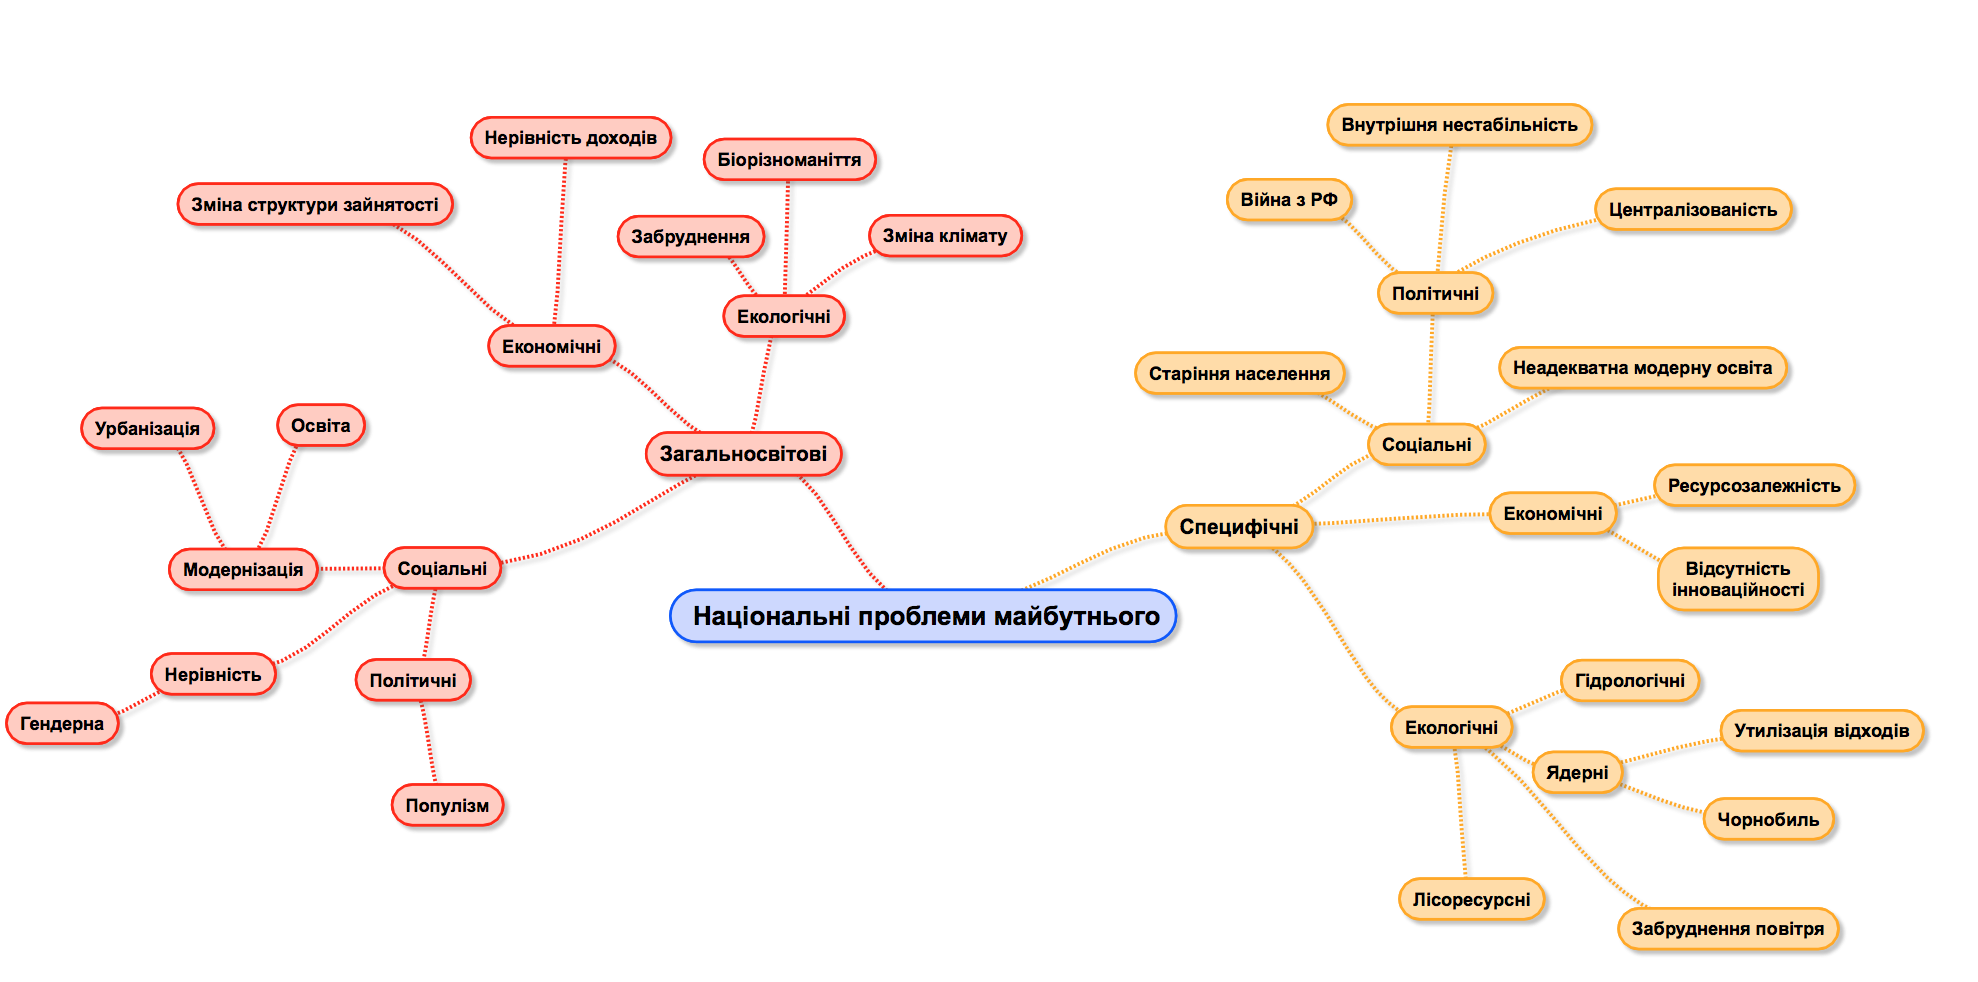
\includegraphics[scale = 0.5]{PNG/mindmap.png}
            \caption{Mind map}
            \label{fig:mindmap}
        \end{figure}

        Окреслимо деякі обрані проблеми більш детально у подальших підрозділах.

    \chapter{Загальнолюдські проблеми}\label{sec:world}


    \section{Зміна структури зайнятості}

        Завдяки прискоренню НТП (науково-технічного прогресу) все більше і більше процесів 
        у нашому житті стають автоматизованими. Машина здатна виконувати багато людських задач так само або краще,
        при цьому із констистентною продуктивністю та не потребуючи заробітньої платні(якщо, звісно, не вважати такою плату за
        спожиту електроенергію). Це, природньо, може призводити до повного або часткового зменшення кількості робочих місць для
        людей у окремих галузях.

        Журнал The Economist наводить інфографіку \cite{econinfo} кількості робочих місць у Сполучених Штатах Америки залежно від типу зайнятості
        з розбивкою по роках. Як типи зайнятості(типи виконуваної роботи) виділяються наступні:

        \begin{itemize}
            \item Рутинна розумова
            \item Рутинна фізична
            \item Нерутинна розумова
            \item Нерутинна фізична,
        \end{itemize}

        де під рутинною мається на увазі одноманітна тощо.

        % \begin{wrapfigure}{r}{0.5\textwidth}
        %     \begin{center}
        %       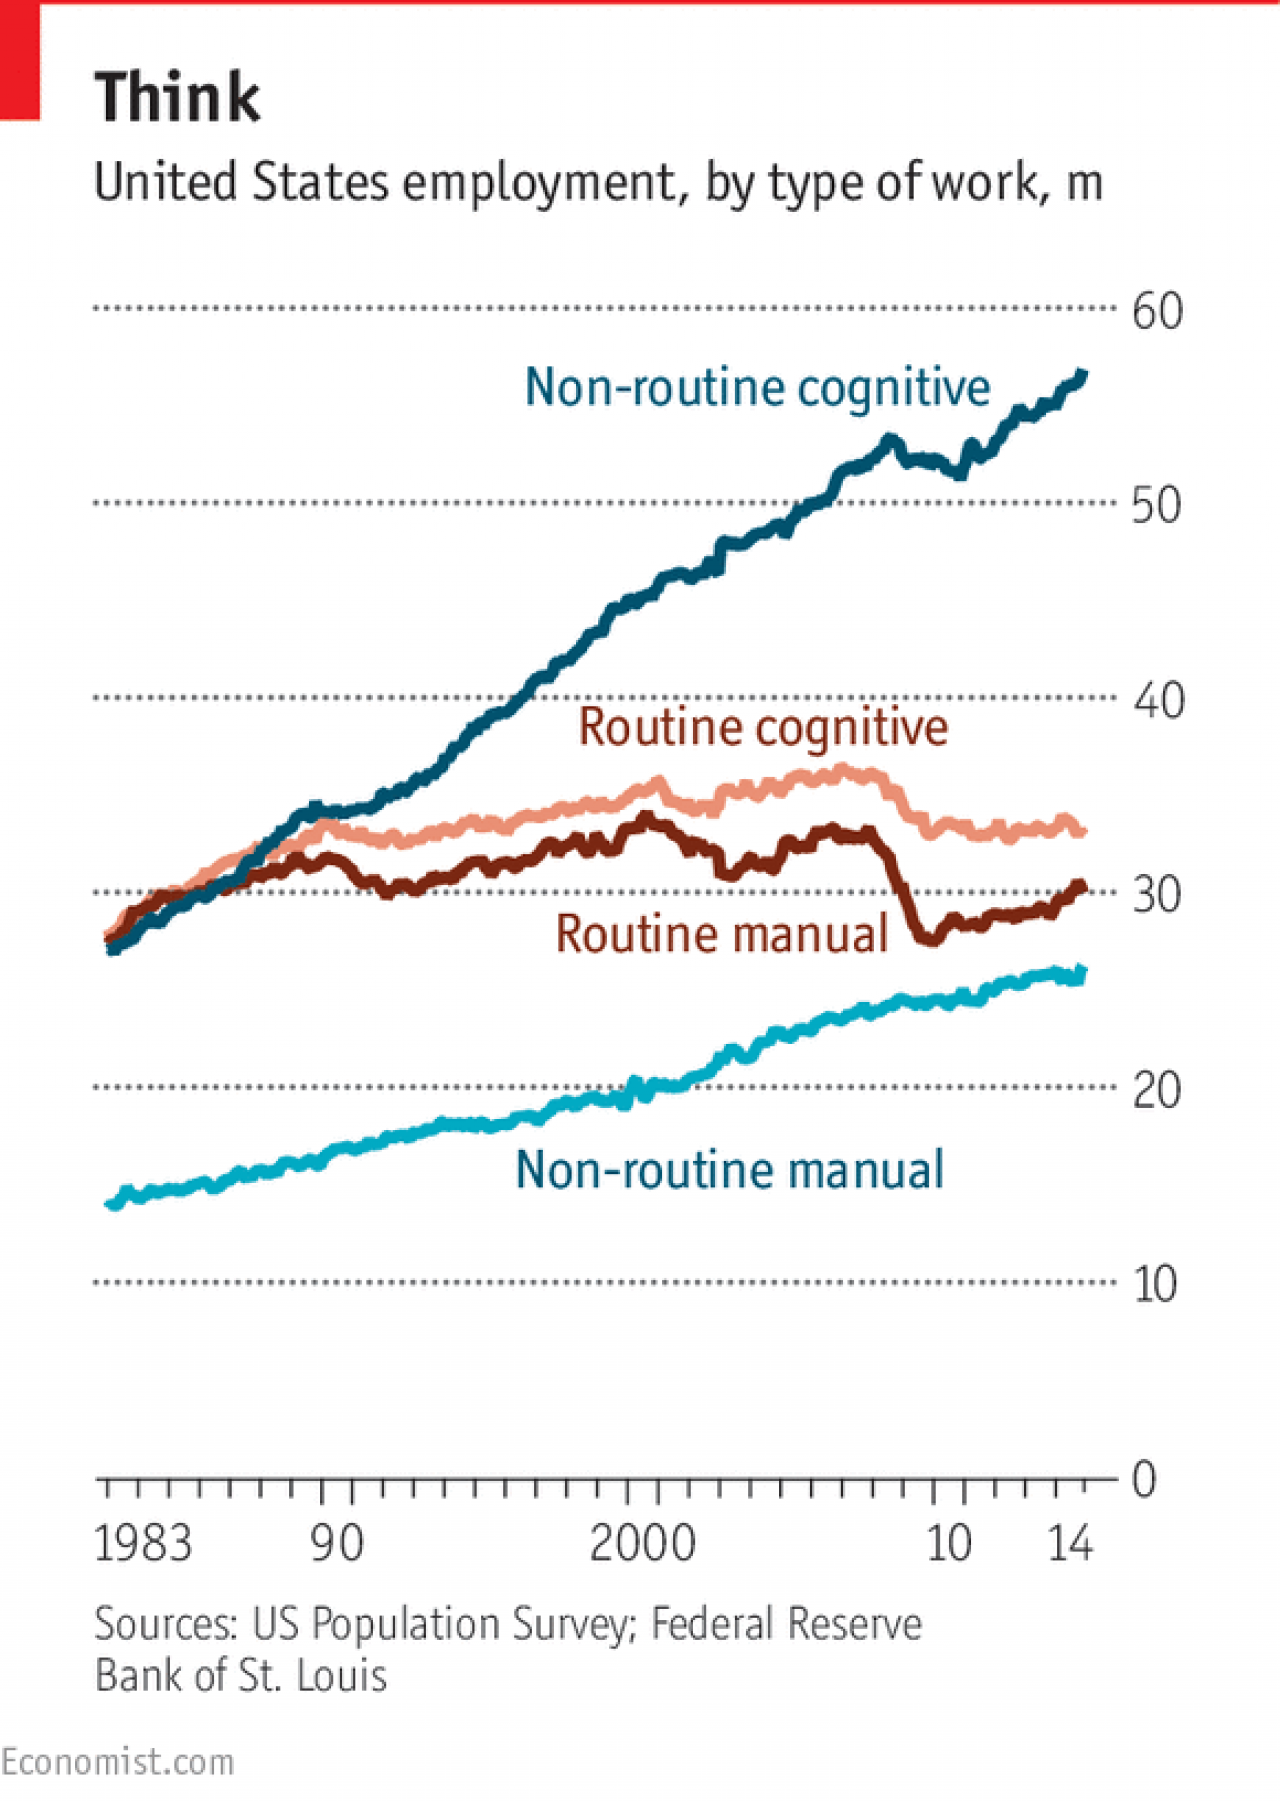
\includegraphics[width=0.48\textwidth]{PNG/economist.png}
        %     \end{center}
        %     \caption{Інфографіка The Economist}
        %     \label{fig:economist}            
        %   \end{wrapfigure}
          

        \begin{figure}[!htp]
            \centering
            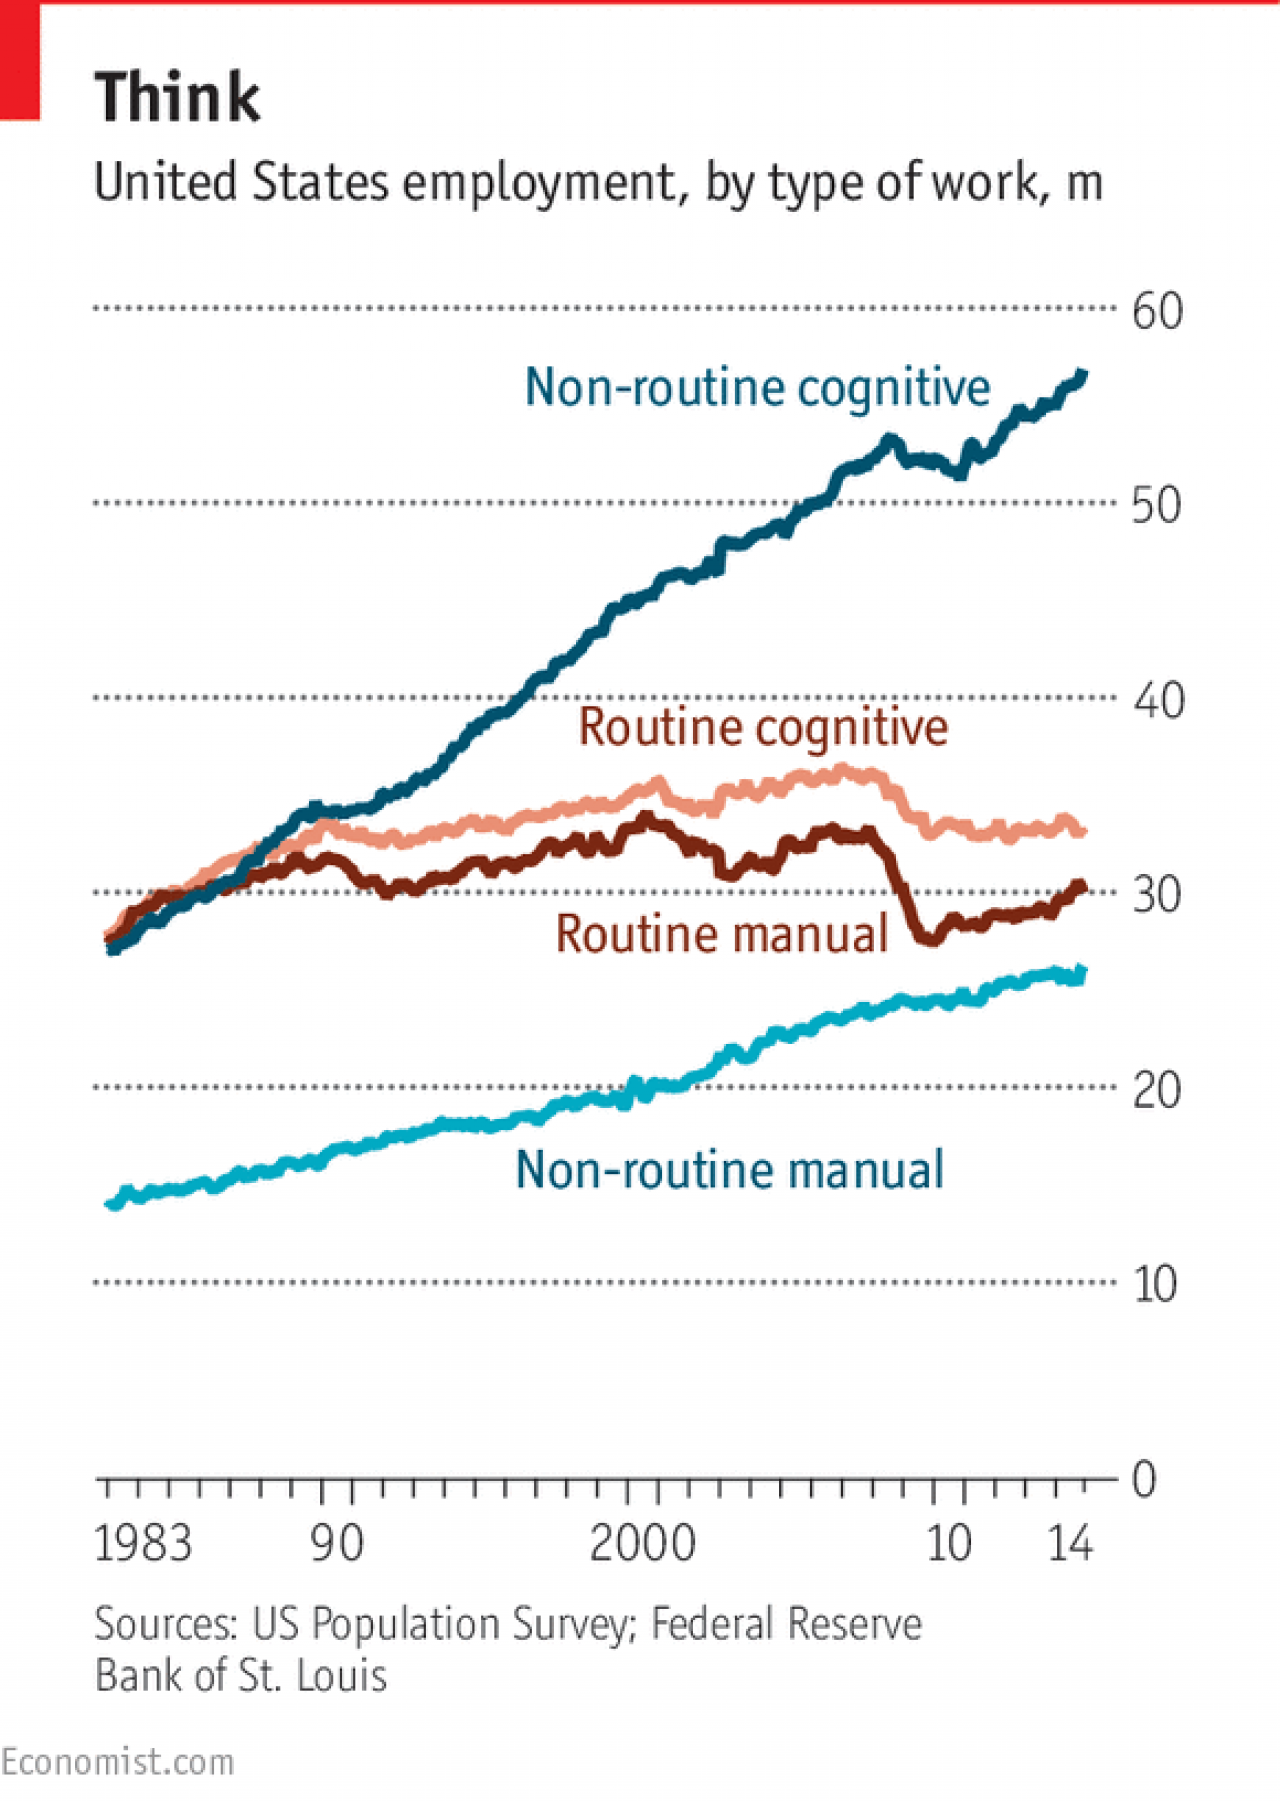
\includegraphics[scale = 0.19]{PNG/economist.png}
            \caption{Інфографіка The Economist}
            \label{fig:economist}
        \end{figure}

        З цієї інфографіки, яку можна побачити на рисунку \ref{fig:economist}, видно, що обсяги рутинних робочих місць перестають
        рости і навіть падають, у той час як обсяг нерутинних загалом не виявляє таких тенденцій. Доповідь PwC (PriceWater Coopers) 
        \cite{pwc} свідчить, що на початку 2030-х років 38 відсотків робочих місць у Сполучених Штатах будуть знаходитись під
        загрозою автоматизації.

        Враховуючи структуру зайнятості України \cite{ukrstatemployment}, для нашої країни ця проблема є ще більш нагальною. 
        Оскільки більшість населення працює фактично на рутинних роботах, можлива автоматизація має потенціал боляче вдарити по нашій
        економіці.

    \section{Зростання нерівності у доходах}
        
        Значною мірою зростанню соціальної напруженості сприяє нерівність у доходах населення. На рисунку \ref{fig:income_us}
        зображена астка доходів верхнього 1-го проценту людей у США по роках. Можна побачити наявність чіткого тренду на її зростання,
        тобто на зростання кількості ресурсів, якими володіє лише один відсоток населення (Зараз він становить майже 20\%)

        \begin{figure}[!htp]
            \centering
            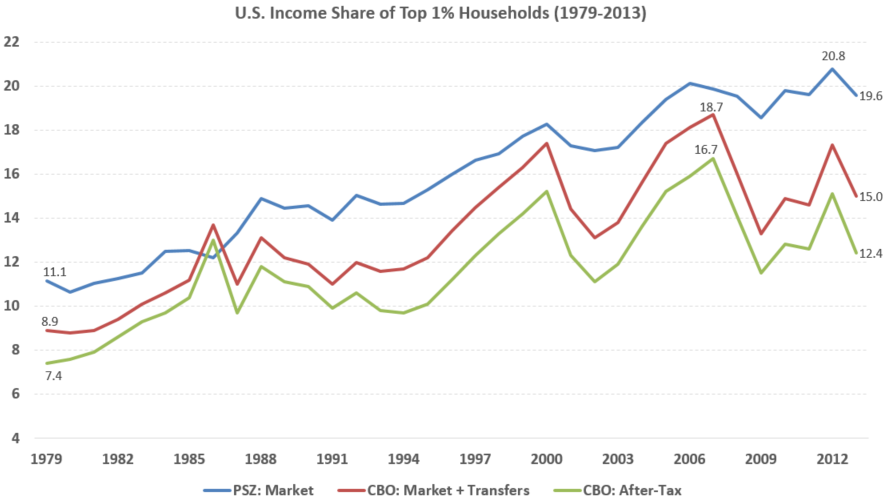
\includegraphics[scale = 0.7]{PNG/income_us.png}
            \caption{Частка доходів верхнього 1-го проценту людей у США по роках}
            \label{fig:income_us}
        \end{figure}

        Хоча нерівність в Україні поки що не показує динаміку до зростання (індекс Джині лишається стабільним, і навіть зменшується
        \cite{giniukr}), ця тенденція може не обминути стороною і нашу країну у майбутньому.

    \section{Змiна клiмату}

        У період з 1950 до 2016 року середня температура на Землі збільшилась на 1 градус \cite{nasa},
        що можна побачити на рисунку \ref{fig:globaltemp}. Ця аномальна як на звичну поведінка 
        приголомшливою більшістю вчених \cite{nasacons} пояснюється зміною клімату внаслідок людської діяльності.
        Обсяги СО2 у атмосфері зростають
        у першу чергу завдяки порушенню балансу через використання викопних джерел енергії. 

        \begin{figure}[!htp]
            \centering
            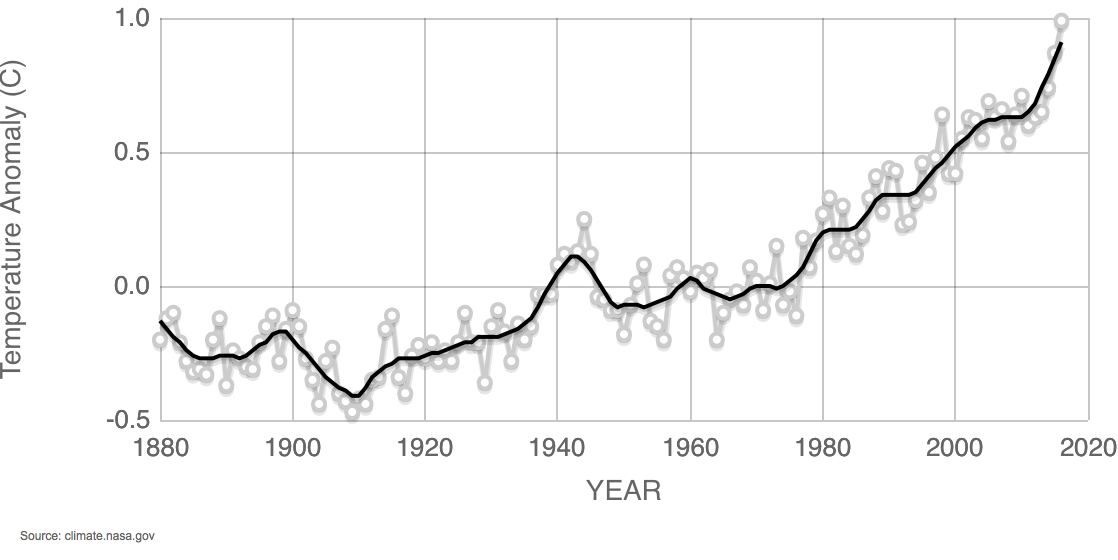
\includegraphics[scale = 0.4]{PNG/GlobalTemp.png}
            \caption{Відносна до 1950 року середня глобальна температура}
            \label{fig:globaltemp}
        \end{figure}

        Незважаючи на думку наукової спільноти, велика кількість політиків відмовляється визнавати зміну клімату і навіть будує на цьому
        кар'єру. Президент чи не найбільшого забрудника - США - Дональд Трамп декілька разів публічно відмовлявся вірити у таку зміну (ц).
        Оскільки ця проблема не має меж і кордонів, для України вона теж є винятково важливо в тому числі і через те, що на наш добробут
        можуть напряму повпливати інші країни.

    \section{Зростання політичного популізму}

        Згадавши про Дональда Трампа, можна згадати і про одну з проблем, які він уособлює "--- зростання політичного популізму 
        по всьому світу. Окрім виборів Трампа можна згадати про вихід Великої Британії із Європейського Союзу (Brexit),
        Вибори президента у Австрії, підйом правих партій Le Front Nacional (Національний фронт) у Франції та AfD 
        (Alternative für Deutschland, ``Альтернатива для Німеччини'') у Німеччині. Всі ці політичні сили об'єднує 
        так званий політичний популізм --- напрям, що орієнтується на пересічного громадянина, часто за допомогою 
        позитивного для такої людини контрасту з деякою елітою (уявною чи абстрактною). Сучасні соціальні мережі 
        та способи поширення новин та думок сприяють створенню так званих ``бульбашок'', у яких поширюються однотипні
        думки. Це є сприятливим середовищем для зростання популістичних рухів. Риторика популізму зазвичай не підкріплена
        фактами, емоційна.

        Втім, не тільки соцмережі становлять проблему. В Україні історично популістичні кандидати отримували великі
        відсотки на виборах, і перемагали на них \cite{Elections}. Але за умови сповзання наших умовних політичних 
        орієнтирів за кордоном до популістичної риторики, замкненої на собі політики, нам стане набагато складніше 
        долати цю перепону в нашій країні.

        \section{Гендерна нерівність}

    \chapter{Специфічно українські проблеми}\label{sec:ukraine}
        \section{Ресурсозалежність}

        Структура української промисловості і, зокрема, експорту, є ресурсоорієнтованою. У 2016 році 
        24 відсотка експорту становили чорні та кольорові метали, ще 45 - продовольчі товари та сировина
        \cite{export2016}. Відповідно, зміни цін на світових ринках (а ресурсні товари є дуже волатильними)
        майже завжди несуть собі потрясіння для української економіки. Наприклад, так було під час світової фінансової
        кризи, коли різко сповільнився \cite{chinagdp} зріст економіки Китаю (рисунок \ref{fig:china}), що призвело
        до значного падіння ціни на чорні метали, що становили основу українського експорту на той час. Іншим
        прикладом згубної ресурсозалежності є зав'язані на нафту економіки Венесуели та Росії,
        які переживають не найкращі часи після різкого обвалу цін на нафтопродукти у 2014 році \cite{brent}.

        \begin{figure}[!htp]
            \centering
            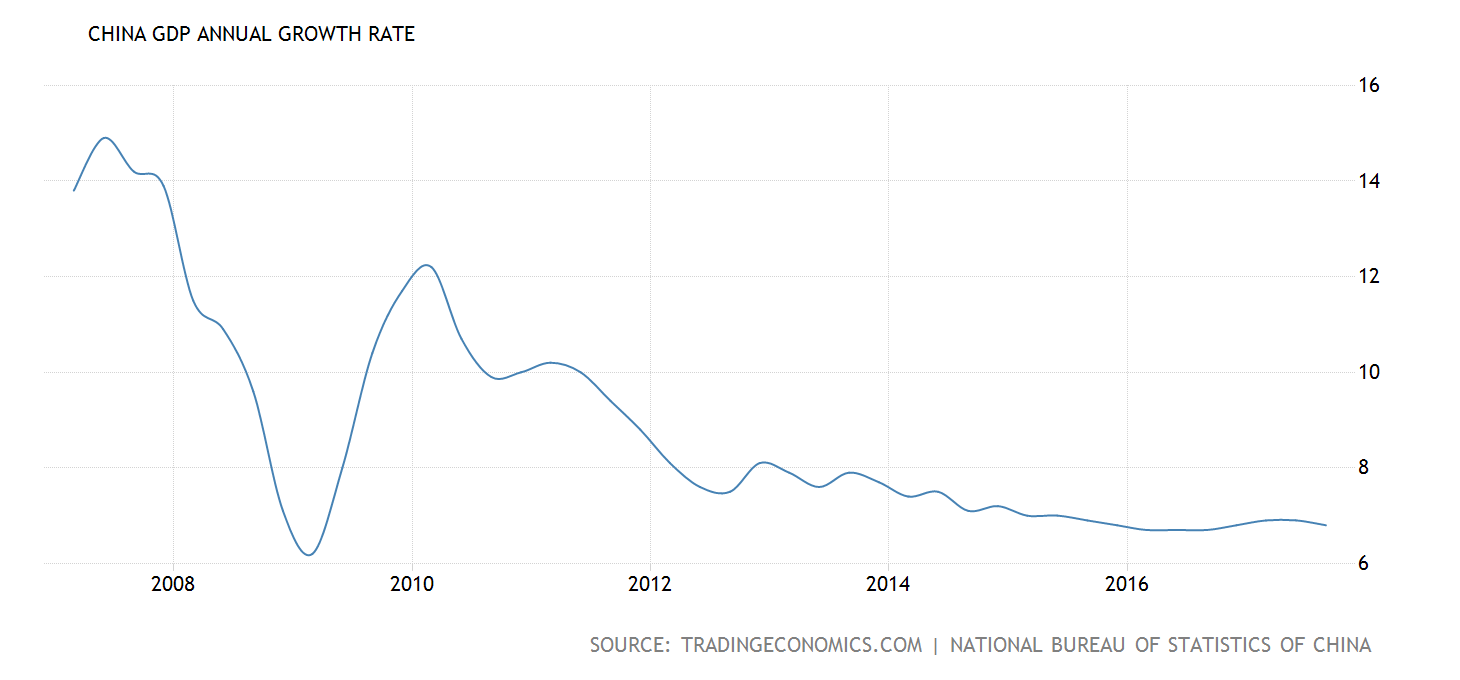
\includegraphics[scale = 0.4]{PNG/china.png}
            \caption{Зростання економіки Китаю, \%}
            \label{fig:china}
        \end{figure}

        Для уникнення подібних ризиків варто змінювати структуру експорту на продукти з більшою доданою вартістю,
        такі як устаткування, ІТ та консультаціні послуги. Втім, незважаючи на зростання цих галузей у експорті \cite{export2016},
        вони все ще становлять мізерну частину від експорту ресурсного.


        \section{Старіння населення та еміграція}
            Досить довгий період населення України старішає (рис \ref{fig:age59}, \ref{fig:age14}). Рівень народжуваності станом на (х) становив (х) (ц). 
            За прогнозами (х) у (х) році в Україні буде (х) людей. Ці показники, втім, не враховують незареєстровану в 
            Україні трудову міграцію. За непрямими джерелами можна оцінити її масштаби. Так, у 2016 році серед вперше отриманих
            робочих віз в ЄС кількість таких, що були отримані українцями, склала близко 600 тисяч (ц). Хоча частина таких
            віз передбачає сезонну роботу, та й частина тих, що виїхали на постійне місцепроживання на кілька років, теж
            повертається, все ж можна скласти уявлення про еміграцію українців. Окрім простого зменшення чисельності населення,
            еміграція становить проблему з двох причин: зменшення кількості працездатного населення --- оскільки саме такі і
            виїзжають, та неповернення до країни активних людей, що могли б змінювати щось всередині держави.

            \begin{figure}[!htp]
                \centering
                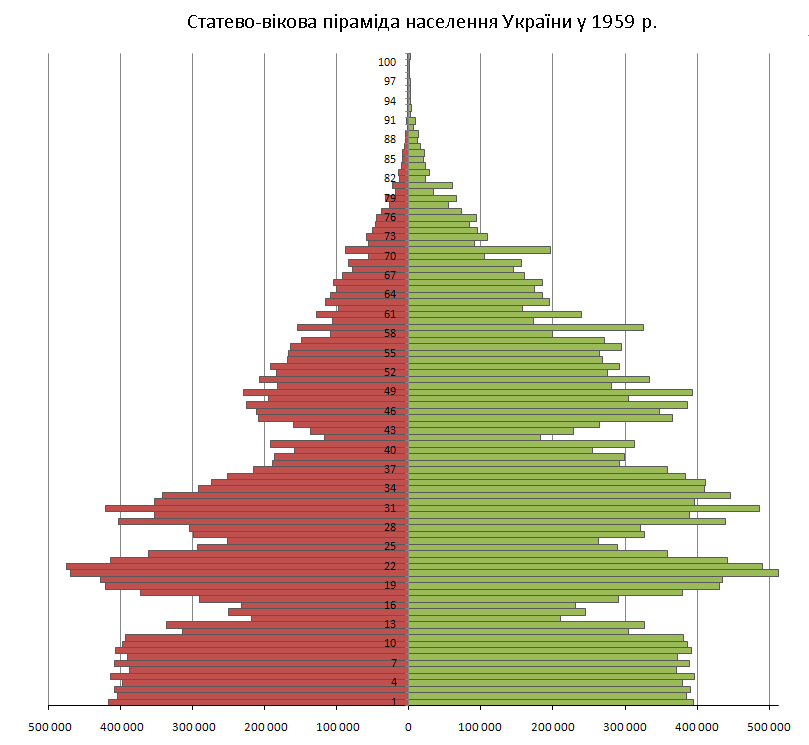
\includegraphics[scale = 0.4]{PNG/PopulationPyramideUkraine1959.PNG}
                \caption{Статево-вікова піраміда населення України у 1959}
                \label{fig:age59}
            \end{figure}

            \begin{figure}[!htp]
                \centering
                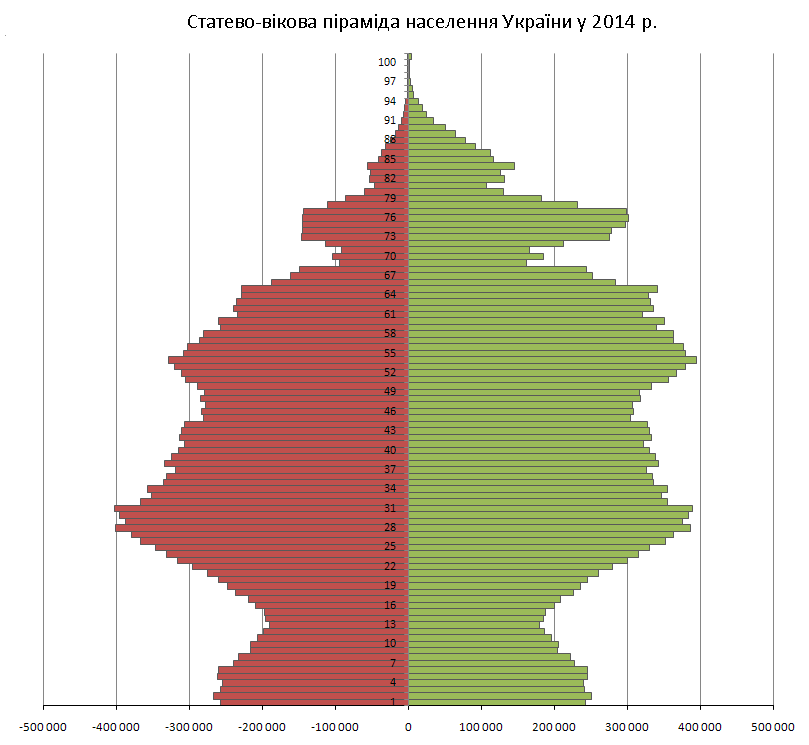
\includegraphics[scale = 0.4]{PNG/PopulationPyramideUkraine2013.PNG}
                \caption{Статево-вікова піраміда населення України у 2014}
                \label{fig:age14}
            \end{figure}

        \section{Забруднення}